% !TEX TS-program = PDfLaTeX
% !TEX encoding = UTF-8
%%
%% AUTORZY szablonu - proszę nie kasować tego komentarza
%Wykonali: Klaudia Olszewska, Natalia Smolińska, Oleksandra Koval, Krzysztof Bielas
%%
\documentclass[12pt,a4paper,oneside]{mwrep}
\usepackage[utf8]{inputenc}
\usepackage[T1]{fontenc}
\usepackage[polish]{babel}
\usepackage[unicode]{hyperref}	

\setlength{\parindent}{4pt}
\setlength{\parskip}{1ex plus 0.5ex minus 0.2ex}

					%W poniższych komentarzach (oznaczonych czerwonym kolorem) znajdują się instrukcje według,
                 					%których należy postępować. Sprowadzają się do wpisywania prostych danych.	
                     				%W nawiasy klamrowe są już wpisane przykładowe dane, które należy zmienić według własnego
\frenchspacing						%uznania.
\usepackage{indentfirst}										%POZOSTAŁEGO KODU NIE NALEŻY ZMIENIAĆ
\usepackage{graphicx, color}
\usepackage{tabularx}
\usepackage{colortbl}	
\usepackage[abs]{overpic}
\usepackage{xcolor,varwidth}
\usepackage{multirow}
\usepackage{caption}	
\usepackage[final]{pdfpages}
\usepackage{lipsum}
\usepackage{url}
\usepackage{float}



%%\usepackage{bookman}              %%  chcąc zmienić font, odkomentuj ta linię
\newcommand{\linia}{\rule{\linewidth}{0.5mm}}	
\makeatletter
\usepackage[top=2cm, bottom=2cm, left=3cm, right=2cm]{geometry}		
\renewcommand{\maketitle}{\begin{titlepage}

	\begin{center}
\huge{\textbf{WYŻSZA SZKOŁA ZARZĄDZANIA \\ ,,EDUKACJA"}}\\[2mm]
	\large {Wydział Zarządzania}\\
	\large {Kierunek:}
	\large												%W poniższy nawias klamrowy wpisz małym literami NAZWĘ KIERUNKU
	 															{informatyka}	
	\end{center}
	\vspace*{3cm}	
	\begin{center}
		\begin{minipage}{8cm}\textbf{}
		\centering
		\textit{}\\
		\Large \textsc{\@author} \\
		\Large {\textsc {Numer albumu:}
		\textsc										%W poniższy nawias klamrowy wpisz NUMER ALBUMU
																{24783}
		}
		\end{minipage}
	\end{center}
	\vspace{2cm}
	\begin{center}	
			\huge
		 	\MakeUppercase{\textbf{\textsc{\@title}}}\\
			\vspace*{0.2cm}
			\large \textbf {Praca} 		
			\MakeLowercase{\large \textbf						%W poniższy nawias klamrowy wpisz  co to jest za praca.
																{Inżynierska}
			}													
	\end{center}
				
	\vspace{3cm}	
	\begin{flushright}
	\begin{minipage}{8cm}
		\begin{flushleft}
		{\large Praca napisana \\ pod kierunkiem naukowym:}\\
		\vspace{0.3cm}
		\Large											%W poniższy nawias klamrowy wpisz tytuł,imię i nazwisko promotora.
																{dr inż. Piotra Grobelnego}
		\end{flushleft}
	\end{minipage}	
	\end{flushright}
	\vspace*{\stretch{10}}
	\begin{center}
		%%\today
Wrocław 2020
	\end{center}	
\end{titlepage} %
}
\makeatother	
\author												%W poniższy nawias klamrowy wpisz imię i nazwisko autora.
																{Grzegorz Dzikowicki}
																
																
\title 													%W poniższy nawias klamrowy wpisz temat pracy.
														{Projekt gry komputerowej z wykorzystaniem silnika Unity}
%%
%%%%Rozdziały biegnące ciurkiem%%%%zakomentuj poniższe linie, jesli chcesz, aby rozdziały zaczynały się od nowej strony%%%%%
\SetSectionFormatting{chapter}
{48pt plus5pt minus2pt}
{\FormatHangHeading{\Large}}
{24pt plus3pt}
%%%%%%%%%%%%%%%%%%%Koniec macra Rozdziały biegnące ciurkiem%%%%%%%%%%%%%%%%%%%%%%%
%%
%%definicje własnych kolorów
\definecolor{kolor}{cmyk}{0.15,0.78,1,0.04}
\definecolor{kolor2}{cmyk}{0.15,0.78,1,0.09}
%%

\pretolerance=1000  %%% globalne ustawienie dzielenia wyrazów na końcu linii; wyższa wartość 'zabrania' dzielenia

\newenvironment{Table}
{\par\medskip\noindent\minipage{\linewidth}}
{\endminipage\par\medskip}
%%
\begin{document}
\maketitle
\baselineskip=19pt  %%%% odstępy międzywierszowe
%%
\tableofcontents
\newpage
\setcounter{page}{2}
\normalsize\rmfamily
\baselineskip24pt
%%
\chapter*{Wstęp}
%%
\begin{quotation}
\indent Gry komputerowe już od wielu lat kreują nowe trendy. Istnieją różne rodzaje gier.
Gry typu AAA tworzone przez wielkie studia gier jak np. Ubisoft, Electronic Arts, czy też nasz rodzimy CD Project Red. 
Patrząc na gry komputerowe klasy AAA możemy śmiało powiedzieć, że przypominają filmy rodem z Disney'a czy też Pixar'a. 
W dzisiejszych czasach, aby oszczędzić sobie czasu, wiele dużych studiów używa technologii Motion Capture, aby odwzorować idealnie ruch postaci. Sprawia to,
<<<<<<< HEAD
że potrzeba manualnego animowania postaci przestaje być kłopotem grafików, oraz animatorów, którzy mogą skupić się na innych aspektach swoich zadań.

\indent Gry typu Indie to produkcje, które zazwyczaj są tworzone przez jedną osobę, bądź amatorskie studio złożone z kilku osób. Ze względu na brak funduszy oraz wyposażenia studia, produkcje te zazwyczaj są niskiej jakości, bądź średni czas potrzebny do przejścia gry jest o wiele krótszy niż gry AAA. Już dekadę temu, wielu graczy zmieniło upodobania co do grafiki, jaka pojawia się w grach komputerowych. Nawiązania do gier z przed dekady uwarunkowane są sentymentem do tamtego okresu. W 2019 do nagrody Paszportu Polityki 2019 została nominowana gra Dawida Ciślaka "We. The Revolution" ~która ukazuje nasze spory wokół sądów i polityki, jednakże podczas czasów rewolucji francuskiej. W dzisiejszych czasach istnieje dużo gier, których grafika składa się z pikseli, voxeli czyli sześciokątów oraz w stylu low-poly który zostanie wykorzystany do tego projektu.

\indent Low-poly jest to angielski termin określający siatkę modelu 3D, która składa się z małej liczby poligonów. Twórcy gier uważają, że low-poly stało się prekursorem grafiki gier komputerowych u dużej ilości osób rozpoczynających swoją przygodę z tworzeniem gier komputerowych. Wykonanie każdego obiektu jest o wiele prostsze od modeli 3D przedstawiających realistycznie postać człowieka bądź drzewa. Ten styl graficzny posiada też swój urok, który można nazwać stylem kreskówkowym. Obiekty są wyraźnie zaznaczone i posiadają cechy charakterystyczne, które pozwalają odróżnić je od innych elementów rozgrywki.
=======
że potrzeba manualnego rigowania postaci --- ustawienia ruchu postaci w sposób realistyczny --- przestaje być kłopotem grafików, oraz animatorów, którzy mogą skupić się na innych aspektach swoich zadań.

\indent Gry typu Indie to produkcje, które zazwyczaj są tworzone przez jedną osobę, bądź amatorskie studio złożone z kilku osób. Ze względu na brak funduszy oraz wyposażenia studia, produkcje te zazwyczaj są niskiej jakości, bądź średni czas potrzebny do przejścia gry jest o wiele krótszy niż gry AAA.
W dzisiejszych czasach istnieje dużo (pełno to kolokwializm) gier, których grafika składa się z pikseli, voxeli czyli sześciokątów oraz w stylu low-poly który zostanie wykorzystany do tego projektu.
>>>>>>> 50ed26ecdf0053dd6ea854a744027c8c69c43bb6

\newpage 
\end{quotation}

%%

%\input{przeg_lit.tex}
%%
\chapter{Cel pracy, wymagania użytkownika, założenia, zakres i~tezy pracy}
%%
\section{Cel pracy}\label{cel}
%%
Celem pracy jest stworzenie projektu gry komputerowej za pomocą silnika Unity której grafika będzie reprezentowała styl graficzny ,,low-poly$"$.
%%

%%
\section{Wymagania użytkownika}
%%
Przez użytkownika (zamawiającego) zdefiniowane zostały następujące wymagania:
\begin{itemize}
\item gra musi być stworzona w środowisku Unity,
\item projekt musi być przedstawiony w formie 3D,
\item gra powinna posiadać świat przedstawiony w postaci low-poly.
\end{itemize}
%%
%%
%%
\section{Założenia}
%%
Przy realizacji projektu przyjęto następujące założenia:
\begin{itemize}
\item do projektu należy stworzyć modele 3D samochodu oraz przeszkód,
\item do projektu należy zaprogramować skrypty obsługujące sterowanie pojazdem oraz mechanikę związaną z przechodzeniem poziomów gry.
\end{itemize}
%%
%%
%%
\section{Zakres}
%%
Zakres pracy obejmował:
\begin{itemize}
\item elementy modeli ze względu na braki funduszy, zostały stworzone w programie Blender,
\item pracę ograniczono jedynie do pięciu krótkich poziomów, ze względu na aktualny stan projektu oraz komplikacje związane z rozmiarem.
\end{itemize}
%%
%%
%%
\newpage
\section{Teza pracy}
%%
Na podstawie przeglądu literatury dotyczącego zagadnienia przyjęto następujące tezy pracy:
\begin{itemize}
  \item do prawidłowego zrealizowania projektu wystarczające jest środowisko Unity, Blender oraz.
\end{itemize}
%%
%%
\chapter{Badania własne}
\begin{quotation}
\indent Proces badawczy to proces planowego, celowego wykorzystania uzyskanych informacji oraz własnej wiedzy. Celem głównym pracy jest próba stworzenia projektu świata przedstawionego w stylu graficznym low-poly. Głównym problemem jest rozmiar gry i złożoność poziomów. Zadecydowano więc, że projekt będzie przedstawiał pięć poziomów, w których gracz musi omijać przeszkody aby przejść na poziom wyżej.

\indent Przeprowadzając badania własne, postanowiono zapoznać się z rynkiem narzędzi służących do tworzenia grafiki 3D. Wybrano 3DS Max, Autodesk Maya, Cinema 4D, ZBrush, Blender oraz Houdini.

\indent Przeszukując możliwe silniki i oprogramowania do tworzenia gier, zdecydowano zaznajomić się z programami RPG Maker, GameMaker, Unreal Engine oraz Unity.
%%
\section{Program do modelowania 3D}

\indent Rynek programów służących do modelowania 3D jest nastawiony na specyficzne projekty. Każde oprogramowanie wybierane jest pod projekt i najczęściej są to programy, które posiadają reputację niezniszczalnych programów, które są niezawodne. Jeżeli firma zajmuje się projektem, który posiada nieprzekraczalny termin dostarczenia, pewnym jest, że wybierze program, który posiada wsparcie konsumenta. Jest to jedna z głównych przyczyn, dlaczego takie programy jak Blender, które są wolnym i otwartym oprogramowaniem, nie są wybierane, ponieważ nie posiadają personelu zajmującego się awariami. Każdy artysta ma swój ulubiony program. Często jest tak, że kierownik projektu z góry narzuca oprogramowanie. Obecnie, do modelowania 3D, animowania, efektów specjalnych oraz rzeźbienia jest używane przynajmniej 5 programów, które nie każdy może znać. Wywiera to presję na artyście. Nie może on skupić się na pracy, ponieważ musi nauczyć się obsługi oprogramowania, które prawdopodobnie zmieni się przy kolejnym projekcie. Wymóg znajomości większości programów do modelowania 3D stał się priorytetem podczas zatrudniania nowego personelu.

\indent 3DS Max jest znany już od dawna. Pierwsza wersja programu ukazała się w 1996r pod nazwą ,,3D Studio Max 1.0''. Posiada bardzo silną pozycję na rynku i jest jednym z najczęściej wybieranych programów do tworzenia grafiki 3D. Program jest przystosowany do tworzenia animacji postaci, ze względu na zaimplementowany system, Character Studio. To oprogramowanie jest często używane w firmach zajmujących się filmami, animacjami oraz grami.

\indent Pierwsza wersja Autodesk Maya zadebiutowała w 1998r. Jeżeli grafikowi zależy na efektach specjalnych, Maya jest najbardziej profesjonalnym wyborem. Posiada solidny zestaw narzędzi, który jest nieobecny w niektórych programach. Niestety profesjonalizm idzie w parze z kosztami. Maya jest jednym z programów graficznych, który posiada najbardziej wygórowaną cenę, 200£ miesięcznie. Firmy takie jak Pixar, korzystają praktycznie tylko z Maya, bowiem ich produkcje wymagają jak najlepszych efektów. Jest to jeden z programów który jest wychwalany przez artystów oraz grafików, ponieważ posiada niesamowity wachlarz narzędzi. Poprzez ilość opcji, funkcji oraz mechanizmów jest również bardzo skomplikowany, przez co jego nauka jest bardzo trudna. Duża liczba osób zaczynających przygodę z modelowaniem 3D, często sięga po darmową wersję trial, jednakże po pierwszym spotkaniu z interfejsem jak i trudnościami w stworzeniu czegokolwiek, szybko zostawiają to oprogramowanie w spokoju.

\indent Jeżeli artyście zależy tylko na animacjach, idealnym oprogramowaniem będzie Cinema 4D. Oprogramowanie to, jest prawdopodobnie jednym z najstarszych na tej liście, bowiem pierwsza jego wersja ukazała się w 1990r. Prawdopodobnym jest, że w większości filmów zawierających nienaturalne animacje, których aktor nie dał rady wykonać, znajduje się animacja stworzona w Cinema 4D. 

\indent ZBrush jest programem który jest nastawiony na Sculpting, czyli rzeźbienie. Tworząc zwykłą kulę a następnie modyfikując ją wszelakimi pędzlami, które dodają, bądź odejmują geometrię, jesteśmy w stanie uzyskać rzeźby identyczne jak w rzeczywistości. Jest to idealny program do tworzenia nieruchomych postaci, które przykładowo pozują. Najczęściej jest wykorzystywany do stworzenia obiektu przypominającego jakiegoś aktora lub postać, który następnie jest użyty w reklamie jako statyczna postać. 

\indent Houdini w głównej mierze używany jest do tworzenia obiektów proceduralnych. Są to obiekty, które są tworzone przez funkcje i modyfikatory, które przy różnych ustawieniach wartości mogą ukazać inny wynik. Jest on tańszym wariantem Autodesk Maya, ponieważ graficy używają go do tworzenia animacji na obiektach wcześniej stworzonych w innym programie do tworzenia grafiki 3D. Często Houdini jest też wykorzystywany do animacji obiektów. Niestety nie jest on na tyle dobrą alternatywą dla Autodesk Maya.

\indent Blender z kolei, jest połączeniem każdego ww. oprogramowania. Posiada praktycznie identyczne funkcje 3DS Maxa pod względem modyfikowania siatki meshowej obiektów 3D. Jeżeli chcemy uzyskać delikatne efekty, można spokojnie użyć do tego Blendera, który poradzi sobie dobrze z naszym problemem, chociaż w Maya udałoby się uzyskać ten sam efekt o wiele lepiej. Animacje w Blenderze polegają jedynie wyobraźni autora. Korzystając z wszelakich transformów oraz modyfikatorów, animacje nie stanowią problemu. Rzeźbienie w Blenderze, przy ustawieniach podstawowych jest trudniejsze niż w ZBrush'u. Ponieważ istnieje opcja importowania gotowych pędzli, dopiero po zebraniu dużej ilości narzędzi przystosowanych do jednego celu, jesteśmy w stanie uzyskać praktycznie ten sam efekt co w ZBrushu. W przypadku tworzenia obiektów proceduralnych, Blender radzi sobie bardzo dobrze. Aby uzyskać efekt jaki możemy dostać w Houdini czy Maya, animator musi się solidnie napracować, co nie oznacza, że jest to niemożliwe do osiągnięcia.

\indent Do realizacji pracy wybrano Blendera, ponieważ każdy z elementów rozgrywki jaki ukaże się w grze jest możliwy do wykonania w tym programie. Ponieważ obiekty 3D potrzebne do projektu nie są wymagające, a efekty specjalne jak i animacje są nieobecne, do wykonania modeli wykorzystano program Blender. Tworząc modele w Blenderze w stylu low-poly, najpopularniejszym narzędziem jest Decimate. Opiera się on na redukowaniu ilości vertexów i ścian siatki meshowej, przez co otrzymujemy mniej detaliczny obiekt o zachowanych proporcjach.
%%
\section{Styl grafiki -- Low-poly}

\indent Pierwsza gra, która posiadała ,,prawdziwe'' 3D, Descent ukazała się w 1995r i została stworzona przez wydawcę gier Interplay Entertainment. Grafikę skonstruowano z poligonów i jako jedna z niewielu gier tamtych czasów pozwalała na sześć stopni swobody, czyli możliwość poruszania się postacią w każdą możliwą stronę horyzontalnie i wertykalnie.

\indent Graficy, tworząc obiekty 3D używają sformułowań odpowiednich do tworzonego przez nich kształtu. Trójkąty popularnie nazywane trisami oraz prostokąty, czyli poligony, posiadają odpowiednią dla figury geometrycznej liczbę ścian i vertexów. \textbf{Vertexy}, są to punkty łączenia krawędzi poligonu. Istnieją również n-gony, czyli figury składające się z liczby ścian większej niż 4. W przypadku, kiedy obiekt nie jest animowany, nie ma żadnych przeciwskazań. Należy jednak pamiętać, że w przypadku, gdy obiekt musi być animowany, powinno się unikać takich rozwiązań, ponieważ silniki renderowania grafiki, mają problem z obliczeniem odbicia światła od powierzchni zawierającej więcej niż 4 vertexy.

\indent Oprawa graficzna w grach jest jednym z najważniejszych kryteriów, która wpływa na to, czy ktoś będzie grał w tą produkcję. Gracze są jednym z najgorszych celów marketingowych. Każdy ma inne wymagania oraz upodobania, przez co trudno trafić w większość. Dzisiejsze produkcje twórców zajmujących się produkcjami AAA opierają się na fotorealistyczności. Jak można się domyślić, nie każdemu to pasuje. Spora liczba graczy preferuje gry, które posiadają wygląd przypominający kreskówki. bądź komiksy. Jedną z takich gier jest ,,The Wolf Among Us'' producenta Telltale Games z 2013r. Przedstawia ona świat, w którym są umieszczone postacie z najbardziej znanych baśni, które często ukazują zachowania patologiczne. Główne postacie żyją w Nowym Jorku, jednej z największych metropolii świata.

\indent W przypadku styli graficznych gier komputerowych, możliwym jest wymienienie głównych przedstawicieli. Gry w stylu 3D zachowujące fotorealizm przodują w rankingach popularności, dlatego też największe studia takie jak Electronic Arts czy Ubisoft skupiają się właśnie na fotorealiźmie. Pomniejsze firmy, których produkty nie są rozpoznawalne na całym globie mają inne zdanie. Każdy ich projekt jest innym przedsięwzięciem celowanym w zupełnie inną publikę. Tacy producenci szukają swojego stylu. W przypadku jeżeli ich gra spodoba się sporej liczbie graczy, próbują stworzyć inną grę, która swoją oprawą graficzną będzie przypominać poprzednią produkcję. Nie zmienai to faktu, że duża liczba gier jest ukazana w środowisku trójwymiarowym. Istnieją też zawzięci fanatycy konkretnych rodzai gier.

\indent Gry 2D przeżywają swego rodzaju renesans. Takie gry jak Horace, Stardew Valley, Darkest Dungeon itp. podbijają serca graczy swoją grafiką i historią. Większość z nich posiada bardzo skomplikowane mechaniki, na które 3D nie pozwala, bądź wymagany jest wielki wysiłek. Mechaniki te mają na celu pokazanie odbiorcy, że nie tylko grafika ma ich cieszyć a rozgrywka.

\indent Gry dzielą się w głównej mierze na 3D i 2D. Ale nie każda gra jest równa drugiej. Dochodzą przeróżne style graficzne. Możliwym jest wylistowanie kilku z najpopularniejszych. Cartooning, czyli po prostu komiks, jest mniej popularny niż reszta styli, co nie zmienia faktu, że posiada swój urok. Świetnie wykonane postacie i charakterystyczna czarna kreska tworząca kontur postaci, kolory są bardzo wyraźne.

\indent Flat design, czyli płaskie elementy zawierające kształty geometryczne. Jak każdy ze styli, posiada fanów oraz krytyków. Spora liczba gier na telefony jest stworzona w stylu flat design. Jego całkowitym przeciwieństwem jest styl fotorealistyczny 3D. Popularnie uważanym jest, że ten styl wykorzystują tylko poważne gry. Zaletą jest poziom detali otoczenia jak i postaci. Minusem jest czas pracy nad poszczególnymi elementami, co również czyni ten styl bardzo kosztownym.

\indent Low-poly jest określeniem siatki modelu 3D, który charakteryzuje się małą ilością wielokątów popularnie zwanych poligonami. Poligony są wykorzystywane do tworzenia obiektów 3D. Siatka modelu tworzona jest poprzez łączenie poligonów w jedną spójną całość. Na przestrzeni lat, patrząc na początki gier komputerowych, dzisiejsze miano low-poly róźnie się diametralnie od swoich poprzedników z przed dwóch dekad. Ze względu na o wiele większą ilość poligonów oraz technologię dzięki której tworzenie modeli 3D jest o wiele łatwiejsze, ten styl dalej odbiega od modeli które są nastawione na realizm. Poligony teoretycznie mogą posiadać nieskończoną ilość boków, jednakże silniki renderowania grafiki często napotykają problem z poligonami, których ilość boków jest większą od pięciu, zwłaszcza przy animacjach ukazujących obiekt w ruchu. Nieoficjalnie ustalono, że siatka modelu musi składać się z trójkątów, bądź prostokątów. Aby obiekt w stylu low-poly posiadał detale prawdziwego obiektu, używa się map normalnych i map wypukłości, które cieniują poligony i dodają im dodatkowej geometrii. \\
Mapy pomagają uwydatnić detale, których ze względu na rozmiar ilość poligonów w siatce obiektu, nie da się uwzględnić ręcznie.

\indent Rozwój technologii silników gier umożliwił nowe rozwiązania dla obiektów low-poly. Odkąd silniki oraz technologia obliczeniowa procesorów rozwinęła się w wielkim stopniu, obecne obliczenia są w stanie przedstawić setki tysięcy poligonów w standardowych 25 klatkach. 
W produkcjach AAA low-poly dalej istnieje, jednakże zostało ograniczone do wykorzystywania mniej detalicznych modeli jako forma zmniejszenia jakości oddalonych obiektów. LOD czyli Level Of Detail, definiuje zasięg z jakim dany obiekt posiada jakość detali. Im dalej znajduje się obiekt, tym gorsze odwzorowanie są detali, które nie pobierają tak dużo mocy obliczeniowej w przypadku głównej sceny, przez co gra działą płynnie \cite{1}.

\indent W przypadku kiedy twórca zdecycował, że chce użyć stylu low-poly, nie ma powodu, żeby używać LODa, ponieważ modele 3D w tym stylu zawierają wystarczającą liczbę detali jak i nie wymagają wielkiej mocy obliczeniowej ze względu na małą liczbę krawędzi.

\begin{figure}[hbt!]
\setcaptionwidth{0.75\linewidth}
\centering
  \includegraphics[width=0.75\linewidth]{lowpolytuto.jpg}
  \caption{Przykładowy render wyspy stworzonej w stylu low-poly}\label{rys_1}
  \begin{minipage}[t]{0.75\linewidth}
    \emph{Źródło: YouTube, CG Geek, Low Poly Island | Beginner | Blender 2.8 Tutorial, 2019.}
  \end{minipage}
\end{figure}


\section{Środowisko tworzenia gry}

\indent Tworząc grę, pierwszą decyzją musi być historia, szata graficzna a następnie wybór silnika oraz środowiska w którym będzie tworzona gra. Ponieważ rynek gier przez ostatnie dwie dekady powiększył się, niektóre silniki postanowiły otworzyć się na świat i stały się wolnymi od opłat oprogramowaniami. Silnikiem określa się zbiór gotowych funkcji potrzebnych do stworzenia gry, które często posiadają zintegrowane środowisko. Silnik zajmuje się komunikowaniem pomiędzy poszczególnymi elementami projektu.

\indent Istnieje wiele programów oraz silników do tworzenia gier komputerowych. Wiodące w branży gier studia, takie jak Ubisoft, Electronic Arts, CD Projekt RED korzystają z własnych silników. Osoby, które tworzą gry w pojedynkę, korzystają z gotowych silników, bądź próbują pisać własne. Najpopularniejszymi gotowymi silnikami są Unity oraz Unreal Engine.

\indent RPG Maker wydany przez firmę Degica jest jednym z programów, który pozwala tworzyć proste gry komputerowe, nie wymagając znajomości języka programowania. Jeżeli twórca zapoznał się z programem i nie chce go zmieniać, musi nauczyć się JavaScript aby tworzyć gry o bardziej skomplikowanych mechanikach.

\indent W 1998r zadebiutowała gra Unreal wyprodukowana przez Epic MegaGames i Digital Extremes, która powstała na pierwszej wersji silnika Unreal Engine I. W 2006r ukazała się trzecia wersja silnika Unreal do której licencję wykupiło wiele przedsiębiorstw takich jak Electronic Arts, Activision czy też Ubisoft, które dziś są jednymi z najbardziej szanowanych studiów zajmujących się tworzeniem gier. W 2015r Unreal Engine stał się darmowy dla każdego, kto chciał rozpocząć przygodę z tworzeniem gier. Spora liczba twórców wybiera Unreal Engine ze względu na możliwość kodowania na klockach, które służą do kodowania wizualnego. Ten moduł wykorzystuje się głównie do prototypowania gier, co nie zmienia faktu, że można tak stworzyć całą grę nie pisząc kodu.

\indent Podobnym do RPG Maker jest następny program, GameMaker stworzona przez firmę YoYo Games. Pierwsze wydanie ukazało się w 1999r. Jest to środowisko do tworzenia gier i programów komputerowych, w którym nie jest wymagana znajomość języka programowania. Ponieważ program jest przeznaczony dla osób nie znających się na programowaniu, GameManager posiada wiele gotowych funkcji, przystosowanych pod konkretne zachowania rozgrywki.  Tak jak Unreal, posiada opcję tworzenia skomplikowanych rozwiązań poprzez łączenie funkcji wizualnie. Środowisko posiada wbudowany język skryptowy GML, tj. GameMaker Language, który porzypomina JavaScript. Został on stworzony z naciskiem na tworzenie gier \cite{2}.

\indent Unity ukazało się w 2005r i początkowo był wykorzystywany w filmach, architekturze i symulacjach. W 2015r trafił do darmowej dystrybucji i szybko stało się konkurencją dla Unreal Engine. Dodatkowo Unity posiada Unity Asset Store, czyli sklep z gotowymi modelami, skryptami a nawet całymi projektami gier. Inspektor, czyli okno akcji każdego obiektu jak i całego projektu, pozwala modyfikować zmienne i dodawać nowe komponenty. Zaimportowany obiekt można dowolnie zmieniać, tj. dodać materiał, kiedy np. importowany obiekt był tylko siatką meshową. W przypadku kiedy w skrypcie zakodowano zmienną, której nadano przykładową wartość, twórca podczas testowania jest w stanie zmieniać jej wartość nie modyfikując kodu, również podczas procesu testowania, właśnie w Inspektorze. Do pisania kodu, wybrano Microsoft Visual Studio 2017, ponieważ darmowa wersja programu jest dołączana do pakietu instalacyjnego Unity. Aktualnie jedynym językiem programowania jest C\#, ponieważ silnik Unity posiada gotowe metody i fukcje, które współgrają wyłącznie z tym językiem. 

\newpage
Unity posiada największą z ww. programów ilość platform do exportowania gry, poczynając od komputerów stacjonarnych z Windowsem, Mac'iem, Linuxem aż do telefonów z iOS bądź Androidem. Do realizacji projektu wybrano Unity, ponieważ pozwala on na stworzenie takiej samej gry jak w Unreal, przy mniejszym wkładzie czasowym. 

\end{quotation}
%%
%%
\newpage
\chapter{Metoda zrealizowania pracy}
\begin{quotation}
%%
\indent Realizacja pracy opiera się na opracowaniu kroków, które należy podjąć aby stworzyć świat gry w stylu low-poly. Dodatkowo aby zaprezentować stworzone elementy, zostanie opracowane przedstawienie produktu za pomocą projektu gry komputerowej stworzonej w Unity.
%%
%%
\section{Narzędzia badawcze}
 Tworząc koncepcję projektu, wybrano poniższe narzędzia badawcze:
\begin{itemize}
\item pierwszym narzędziem badawczym do stworzenia obiektów, będzie program Blender, który idealnie nadaje się do tworzenia elementów grafiki 3D,

\item drugim narzędziem badawczym, które posłuży do stworzenia gry komputerowej będzie środowisko Unity, w którym zostaną ułożone podstawowe elementy rozgrywki, takie jak przeszkody,

\item trzecim narzędziem badawczym, dzięki któremu napiszemy kod do gry, będzie Microsoft Visual Studio 2017.

\end{itemize}
%%

\section{Technika tworzenia obiektów 3D}
\indent Obiekty grafiki 3D o mianie low-poly określa się przedmioty, postacie, świat gry itp. na których widać wyraźne elementy trisów bądź poligonów. Są to wyraźnie zaznaczone krawędzie obiektu, które swoją geometrią przypominają odpowiednik w świecie rzeczywistym, które różnią się stopniem skomplikowania obiektu. Aby stworzyć taki model, najłatwiej jest zacząć od projektów poglądowych. W studiach gier, zatrudnieni sią artyści, którzy podczas omawiania aspektów danych postaci bądź elementów świata, rysują proste szkice, które następnie poprawiają w celu uwydatnienia kluczowych aspektów obiektu. 
W późniejszym stadium rozwoju danego elementu, powstaje tzw. szkic końcowy. Wówczas owy szkic przekazuje się osobom, które zajmują się grafiką komputerową aby stworzyli dany obiekt w środowisku 3D. Do projektu użyto zdjęć poglądowych dla beczki, oraz słupka drogowego.

\indent Tworząc obiekt zazwyczaj zaczyna się od zwykłej kostki sześciennej, którą następnie modyfikuje się poprzez przesuwanie vertexów, krawędzi bądź całych ścian obiektu. Istnieje wiele narzędzi w Blenderze, które pomagają uzyskać porządany przez nas efekt takie jak ,Mirror''. Dodając ten modyfikator na obiekt, otrzymujemy odbicie lustrzane ukazujące dwie identyczne połówki. Korzystając ze zdjęcia referencyjnego ustawionego w widoku side view (bocznym) możemy ustawiać krawędzie obiektu nadając mu identyczny kształt jak na zdjęciu. Samochód który będzie głównym pojazdem w projekcie został stworzony za pomocą zdjęcia poglądowego Poloneza oraz własnej wyobraźni, ponieważ jego proporcje oraz kształt są niczym wyjęte z kreskówki. Obiekty stworzone w Blenderze, zostały wyeksportowane jako plik typu fbx.

\begin{figure}[!hbt]
\setcaptionwidth{0.75\linewidth}
\centering
  \includegraphics[width=0.75\linewidth]{carblend.png}
  \caption{Render samochodu stworzonego na potrzeby projektu}\label{rys_2}
  \begin{minipage}[t]{0.75\linewidth}
    \emph{Źródło: Opracowanie własne}
  \end{minipage}
\end{figure}

\newpage
\section{Środowisko Unity}
\indent Po wcześniejszym stworzeniu obiektów w Blenderze, przeniesiono je do środowiska Unity. Aby obiekty nie wisiały w powietrzu, została stworzona płaska powierzchnia o rozmiarach 15x3x1000 jednostek Unity. Następnie umieszczono wszystkie obiekty w scenie. Każdy z obiektów posiada komponenty Mesh Collider, który odpowiada za wykrywanie kolizji z innymi obiektami, oraz Rigidbody będący głównym elementem fizyki obiektów.  Zostały zmodyfikowane ich masy oraz rozmiary aby stworzyć dla nich prefab. Prefabem nazywany jest ten sam obiekt, który po ponownym umieszczeniu w scenie posiada te same właściwości. Ustawiając obiekty na powierzchni, stworzono 5 różnych poziomów, które różnią się trudnością, odpowiednio od pierwszego do piątego. Każdy z nich jest  bardziej skomplikowany. 

\indent Przejścia pomiędzy poziomami będą zawierały krótką i prostą animację wyświetlającą wiadomość ,,LEVEL COMPLETE''. Tworzenie animacji polega na stworzeniu Panelu z tekstem a następnie na osi czasu zmiany wartości alfy, tak aby napis oraz tło pojawiły się. W sekcji programowania znajduje się kod odpowiedzialny za proces przejścia z jednego poziomu na drugi. 

\begin{figure}[!h]
\setcaptionwidth{0.75\linewidth}
\centering
  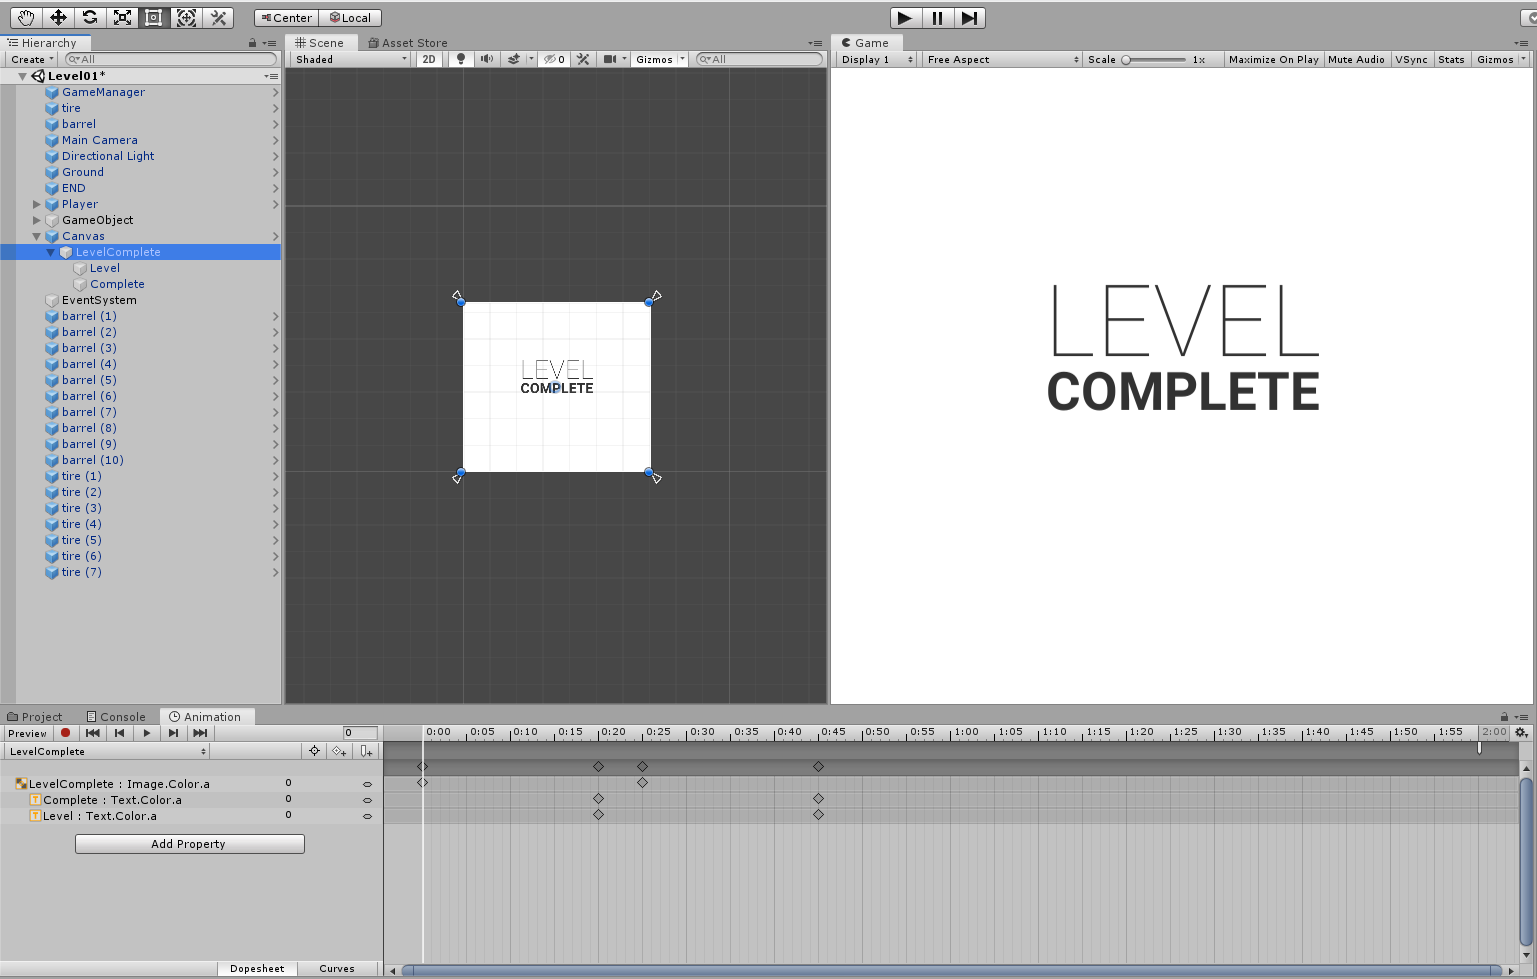
\includegraphics[width=0.75\linewidth]{levelcomplete2.png}
  \caption{Screenshot pokazujący LEVEL COMPLETE, poniżej oś czasu z kluczowymi klatkami tworzącymi animację.}\label{rys_3}
  \begin{minipage}[t]{0.75\linewidth}
    \emph{Źródło: Opracowanie własne}
  \end{minipage}
\end{figure}

\newpage
\section{Programowanie skryptów}
\indent Programowanie zaczęto od stworzenia skryptu obsługującego poruszanie się pojazdem. Aby obiekt się poruszał, wykorzystano komponent Rigidbody umieszczony na samochodzie. Korzystając z gotowych funkcji zawartch w Rigidbody, mianowicie \textit{AddForce()}, można sprawić aby obiekt poruszał się w danym kierunku z określoną mocą.

\begin{figure}[!h]
\setcaptionwidth{0.75\linewidth}
\centering
  \includegraphics[width=1\linewidth]{playermove.png}
  \caption{Skrypt PlayerMovement obsługujący poruszanie się pojazdu po poziomie.}\label{rys_4}
  \begin{minipage}[t]{0.75\linewidth}
    \emph{Źródło: Opracowanie własne}
  \end{minipage}
\end{figure}

\begin{figure}[!h]
\setcaptionwidth{0.75\linewidth}
\centering
  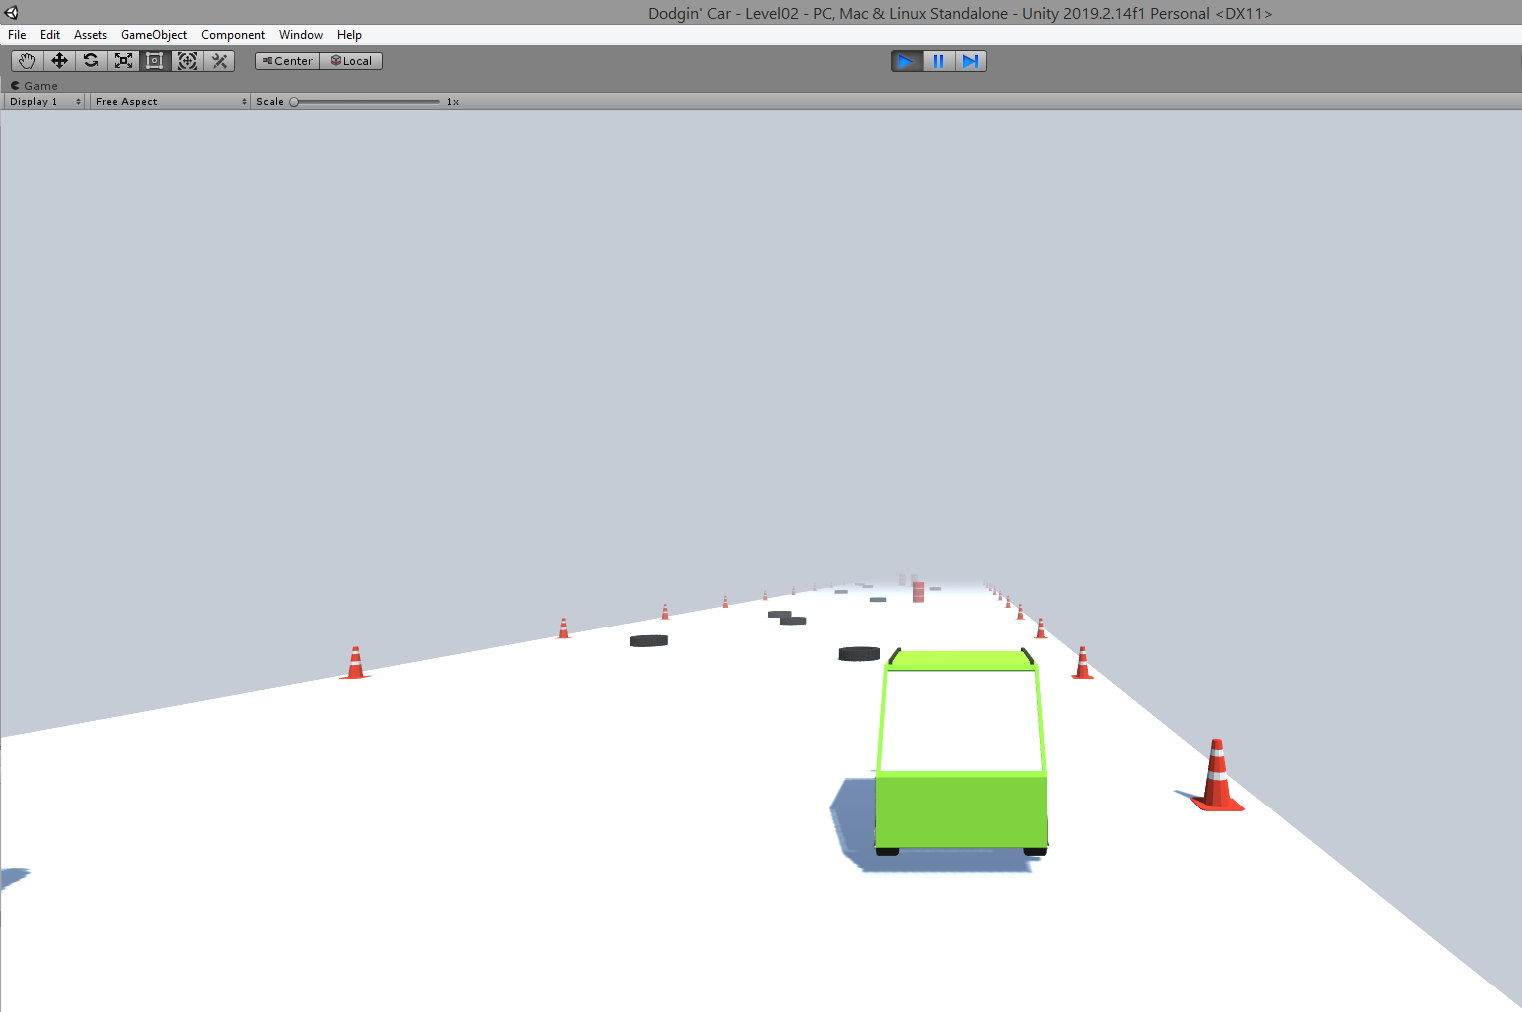
\includegraphics[width=1\linewidth]{playermovelook.png}
  \caption{Zdjęcie ukazujące pojazd, który zboczył ze środka trasy.}\label{rys_5}
  \begin{minipage}[t]{0.75\linewidth}
    \emph{Źródło: Opracowanie własne}
  \end{minipage}
\end{figure}

\newpage
\indent Kamera musi śledzić gracza, dlatego napisano skrypt, który ustala pozycję kamery w świecie gry, na taką samą pozycję co pojazd, jednakże dodany jest offset czyli przesunięcie, które podnosi kamerę do góry i przesuwa ją do tyłu, tak aby widok był z perspektywy trzeciej osoby.

\begin{figure}[!h]
\setcaptionwidth{0.75\linewidth}
\centering
  \includegraphics[width=1\linewidth]{followplayer.png}
  \caption{Skrypt FollowPlayer obsługujący umieszczenie kamery za pojazdem.}\label{rys_6}
  \begin{minipage}[t]{0.75\linewidth}
    \emph{Źródło: Opracowanie własne}
  \end{minipage}
\end{figure}
\indent Kolejnym zadaniem było napisanie skryptu, który będzie wykrywał kolizje z przeszkodami oraz resetował poziom, jeżeli pojazd spadnie z planszy. Ponieważ platforma po której porusza się pojazd, również jest wykrywana jako kolizja, wszystkie przeszkody zostały otagowane jako ,,Obstacle''. W skrypcie PlayerMovement został dodany kod obsługujący resetowanie poziomu, jeżeli wartość y pojazdu spadnie poniżej -1, który odwołuje się do funkcji \textit{EndGame()} w skrypcie GameManager.

\begin{figure}[!hbt]
\setcaptionwidth{0.75\linewidth}
\centering
  \includegraphics[width=1\linewidth]{playercollision.png}
  \caption{Skrypt PlayerCollision obsługujący kolizje pomiędzy pojazdem a przeszkodami.}\label{rys_7}
  \begin{minipage}[t]{0.75\linewidth}
    \emph{Źródło: Opracowanie własne}
  \end{minipage}
\end{figure}
%%
\begin{figure}[!hbt]
\setcaptionwidth{0.75\linewidth}
\centering
  \includegraphics[width=1\linewidth]{gamemanager.png}
  \caption{Skrypt GameManager zajmujący się restowaniem poziomów.}\label{rys_8}
  \begin{minipage}[t]{0.75\linewidth}
    \emph{Źródło: Opracowanie własne}
  \end{minipage}
\end{figure}

\newpage
\hfill \break
\hfill \break
\indent Ponieważ w inspektorze nie da się podpiąć skryptu GameManager do prefabu pojazdu, w skrypcie PlayerCollision znajduje się metoda \textit{FindObjectOfType} która przeszukuje w lokalizacji skryptów plik o nazwie GameManager a następnie korzysta z jego funkcji która musi być ustawiona jako publiczna. Stworzono typ logiczny bool gameHasEnded, który przybiera dwie wartości, prawda lub fałsz, którego wartość zmieniana jest przy pierwszym uruchomieniu funkcji, aby upewnić się, że funkcja będzie ładowana tylko jeden raz. Następnie po upadku, bądź kolizji, poziom jest ładowany od nowa, tak więc gameHasEnded ma swoją pierwotną wartość. Aby gra nie resetowała się za szybko, zamiast uruchamiać funkcję \textit{EndGame()} od razu, wykorzystano metodę \textit{Invoke} która po dodaniu nazwy funkcji, oraz czasu w sekundach, uruchamia funkcję po określonym czasie. Aby przejść na następny poziom, gracz musi przejechać pomiędzy przeszkodami tak żeby ich nie dotknąć. W przypadku porażki poziom zostanie załadowany od nowa.

\indent Poziom jest już możliwy do przejścia, jednakże trzeba załadować kolejny. Na końcu trasy każdego z poziomów umieszczono kostkę o szerokości 15 jednostek Unity, która jest niewidoczna i służy jako przełącznik uruchamiający animację zakończonego poziomu, oraz ładuje kolejny. W skrypcie EndTrigger znajduje się jedna funkcja \textit{OnTriggerEnter()}, która ładuje funkcję \textit{CompleteLevel()} ze skryptu GameManager odpowiedzialną za włączenie animacji zakończenia poziomu.

\begin{figure}[!ht]
\setcaptionwidth{0.75\linewidth}
\centering
  \includegraphics[width=0.8\linewidth]{endtrigger.png}
  \caption{Skrypt EndTrigger nawiązujący do GameManager.}\label{rys_9}
  \begin{minipage}[t]{0.75\linewidth}
    \emph{Źródło: Opracowanie własne}
  \end{minipage}
\end{figure}

\begin{figure}[!h]
\setcaptionwidth{0.75\linewidth}
\centering
  \includegraphics[width=1\linewidth]{loadlevel.png}
  \caption{Skrypt LevelComplete ładujący kolejny poziom.}\label{rys_10}
  \begin{minipage}[t]{0.75\linewidth}
    \emph{Źródło: Opracowanie własne}
  \end{minipage}
\end{figure}

\end{quotation}
%%
%\input{wyniki.tex}
%%%
\newpage
\chapter{Podsumowanie}
\begin{quotation}

\indent Proces tworzenia gier komputerowych wymaga od twórcy poświęcenia czasu na zapoznanie się z historią stylu graficznego oraz jego wymaganiami. Tworząc grę low-poly należy pamiętać, aby modele 3D posiadały siatkę modelu która będzie wykonana poprawnie. Ważnym elementem tworzenia gier w konkretnym stylu jest zebranie informacji dotyczących wymagań topologii modeli. Charakterystyczne cechy stylu low-poly to siatka modelu składająca się z trisów i poligonów prostokątnych. Obiekt nie może posiadać dużej ilości poligonów, ponieważ jak sama nazwa wzkazuje, nie będzie to low-poly. Małe detale trzeba ograniczyć do minimum, bądź całkowicie wykluczyć a kolory obiektów muszą się wyróżniać, aby modele nie nakładały się na siebie. 

\indent Tworząc obiekt, którego pierwowzór ma odzwierciedlenie w rzeczywistości, należy pamiętać aby stworzyć go w taki sposób, aby jak najbardziej przypominał tą rzecz, chociażby pod względem kształtu. Jedno z narzędzi Blendera, Extrude, jest najlepszym przyjacielem twórcy. Za jego pomocą jesteśmy w stanie dowolnie rozszerzać siatkę modelu dodając przy tym dodatkowej objętości. Najczęstszym sposobem na modyfikowanie obiektu jest jego skalowanie. Modyfikując poszczególne elementy obiektu, twórca jest w stanie uzyskać nowe krawędzie, które nadadzą modelowi wymaganej geometrii. Modyfikator Mirror, jest przydatny w momentach, kiedy twórca skupia się na jednej stronie modelu, aby przesuwając i modyfikując konkretną część obiektu, uzyskać idealne odbicie lustrzane. W przypadku gdy twórca chce uzyskać ciekawy efekt wizualny obiektu, zamiast tworzyć ręcznie trisy na siatce obiektu, może użyć modyfikatora Triangulate, który zmodyfikuje siatkę meshową modelu, przerabiając każdy możliwy poligon na dwa trisy. Niestety wiąże się to z konsekwencją zwiększenia ilości poligonów w obiekcie, co może doprowadzić do komplikacji związanych z przewidywaną liczbą ścian w każdym obiekcie.

\indent Umiejętność operowania w danym programie, który służy się do tworzenia gier, również jest przydatna, ze względu na czas. Tworząc obiekty w Blenderze, po wcześniejszym nauczeniu się programu, skrótów oraz dostępnych modyfikatorów, możliwym jest stworzenie modelu w krótkim czasie. Korzystając z silnika gry, który wymaga pisania skryptów, aby uzyskać przeróżne mechaniki rozgrywki, dodatkowo rozwijana jest znajomość języka programowania, użyteczna w następnych projektach. Otrzymanie żądanego efektu może zająć sporo czasu, jednakże podczas powstawania kolejnego projektu, jesteśmy w stanie uzyskać ten sam efekt, bądź lepszy, w o wiele krótszym czasie. Blender jako darmowe oprogramowanie często jest pomijany przez wielkie firmy zajmujące się animacjami oraz modelowaniem 3D. Jest to spowodowane brakiem wsparcia technicznego, które jest wymagane w przypadku, kiedy podczas procesu tworzenia ważnego projektu, wyłączy się program i nie można go uruchomić ponownie, bądź wszystkie dane zostały stracone. Nie zmienia to faktu, że Blender dorównuje swoim konkurentom i prędzej czy później osiągnie status jednego z najlepszych oprogramowań dostępnych za darmo na rynku.

\indent Jak widać w rozdziale \textbf{3.4}, aby stworzyć grę wymagana jest podstawowa wiedza o języku programowania, oraz znajomość funkcji silnika Unity. Wszystkie gotowe funkcje i metody zawarte w silniku Unity są udostępnione w Unity User Manual dostępnym na stronie głównej Unity. Podczas pisania kodu ważnym jest aby zwracać uwagę na pisanie pierwszych liter. C\# jest językiem programowania, który zwraca uwagę na to, czy funkcja jest napisana z dużej litery czy nie. Standardem jest, aby zmienne zaczynały się z małej litery a metody i fukcje z dużej. \\
Istnieją też dwie szkoły pisania długich nazw. Aby oddzielić od siebie słowa korzysta się ze snake'a albo camel'a. \textbf{to\_jest\_snake} czyli oddzielanie słów za pomocą znaku podkreślenia, a \textbf{toJestCamel}, czyli pisanie pierwszego słowa z małej litery, a następnie zaczynanie każdego następnego słowa z wielkiej. 
\indent Należy pamiętać o konieczności przystosowania gry do każdego komputera. Do metod które wpływają na rozgrywkę, takie jak poruszanie się, należy dodać \textit{Time.deltaTime} aby sprzęt na którym się gra, nie dawał przewagi. Poprzez \textit{ForceMode.VelocityChange} twórca jest w stanie uzyskać element prawdziwego poruszana się dwóch różnych obiektów o tej samej prędkości. Dodatkowo ten tryb pozwala uzyskać sposób poruszania się obiektów po scenie w stylu gier typu Arcade.

\indent Spełnione zostały wymagania użytkownika, a teza została udowodniona. Gra została stworzona w środowisku Unity w formie 3D, a modele przeszkód i pojazdu zostały wykonane w postaci low-poly. Plik instalacyjny gry został stworzony w programie Inno Setup a następnie nagrany na płytę. Założenia projektu obejmowały stworzenie modeli 3D oraz zaprogramowanie skryptów obsługujących sterowanie i mechaniki gry. Powstały trzy modele przeszkód oraz jeden pojazd. Podczas procesu programowania powstało 6 skryptów zajmujących się rozgrywką, oraz dwa obsługujące przyciski startu oraz wyjścia z gry. 
\end{quotation}
%%
\newpage
%%
\chapter{Wnioski}
%%
Realizacja pracy pozwoliła sprecyzować następujące wnioski:
\begin{enumerate}
  \item do stworzenia gry 3D w stylu low poly wystarczające jest środowisko Unity,
  \item Blender jest wystarczająco dobrym środowiskiem do tworzenia obiektów 3D.
\end{enumerate}



\begin{quote}
\scriptsize{
\underline{\textcolor{blue}{Objaśnienie:}}\\[1mm]
\textcolor{blue}{{\textbf{Wnioski}:} (lista syntetycznych wniosków)}\\[1mm]
\textcolor{blue}{
Wnioski powinny:
\begin{enumerate}
\item jednoznacznie określać czy i~jak został osiągnięty cel pracy,
\item podsumować w~jaki sposób zweryfikowano hipotezy (jeśli były postawione),
\item odpowiadać na pytanie o~słuszność tez (czy je udowodniono).
\end{enumerate}
}}
\end{quote} 

\renewcommand{\bibname}{Spis literatury}

\bibliographystyle{unsrt}
\bibliography{biblio}
%\begin{quote}
%\scriptsize{
%\underline{\textcolor{blue}{Objaśnienie:}}\\[1mm]
%\textcolor{blue}{{\textbf{Literatura}:} (lista wszystkich przywołań i odwołań)}\\[1mm]
%\textcolor{blue}{
%Spis literatury, tzw. \emph{Bibliografia} powinna zawierać ponumerowany  wykaz - cytowanych w pracy, \textbf{w kolejności cytowania} - publikacji zwartych (książek), materiałów %konferencyjnych, artykułów w czasopismach naukowych, popularnonaukowych, źródeł elektronicznych (np. internetowych) itp. Stosować biblioteczną bazę danych BiB\TeX a oraz styl %cpm.bst.
%}}
%\end{quote}
\chapter*{Załączniki}
%%
\section*{Zał. nr 1  Oświadczenie dotyczące praw autorskich i danych osobowych przechowywanych w Systemie Antyplagiatowym}

\section*{Zał. nr 2 Płyta CD}
\centering
Do pracy dołączono płytę CD z następującą zawartością: 
\hfill \break
\hfill \break
\begin{tabular}{|r|l|} \hline
Katalog & Zawartość \\ \hline
Installer & Plik instalacyjny z grą \\
Praca & Praca inżynierska w formacie PDF \\
Projekt Unity & Folder zawierający projekt wykonany w Unity \\
Pliki Blender & Folder zawierający wszystkie pliki .blend \\ \hline

\end{tabular}


\includepdf[pages=-]{oswiadczenie.pdf}

%%
\end{document}
